\documentclass[rnd]{mas_proposal}
% \documentclass[thesis]{mas_proposal}

\usepackage[utf8]{inputenc}
\usepackage{amsmath}
\usepackage{amsfonts}
\usepackage{amssymb}
\usepackage{graphicx}
\usepackage{booktabs}
\usepackage{float}
%\usepackage[showframe=true]{geometry}
\usepackage{changepage}
\usepackage{lipsum}
\usepackage{array}
\usepackage{makecell}
\usepackage{csquotes}
\renewcommand\theadalign{bc}
\renewcommand\theadfont{\bfseries}
\renewcommand\theadgape{\Gape[4pt]}
\renewcommand\cellgape{\Gape[4pt]}



\usepackage{xcolor}
\usepackage{listings}
\usepackage{caption}
\DeclareCaptionFont{white}{\color{white}}
\DeclareCaptionFormat{listing}{%
	\parbox{\textwidth}{\colorbox{gray}{\parbox{\textwidth}{#1#2#3}}\vskip-4pt}}
\captionsetup[lstlisting]{format=listing,labelfont=white,textfont=white}
\lstset{frame=lrb,xleftmargin=\fboxsep,xrightmargin=-\fboxsep}

\lstset{
	% numbers=left,
	breaklines=true,
	% backgroundcolor=\color{light-gray},
	tabsize=4,
	% basicstyle=\ttfamily,
	literate={\ \ }{{\ }}1	
}


\title{Design and Realisation of Smart Non-prehensile Manipulation Strategies for Robots
}
\author{Pooja Bhat}
\supervisors{Prof. Dr. Nico Hochgeschwender\\Prof. Dr. Paul G. Pl\"oger\\ M. Sc. Sven Schneider \\ Dr. Matthias Nieuwenhuisen}
\date{1 August, 2020}

% \thirdpartylogo{path/to/your/image}

\begin{document}

\maketitle

\pagestyle{plain}

\section{Introduction}
%
    
    %\item An introduction to the general topic you are covering.
        
   % \item Why is it important?
%\end{itemize}
Humans perform skillful manipulation as combined sequences of various motion primitives, in contrast to most robots that are limited to picking and placing the objects by grasping them. For example, a simple door opening task involves grasping and turning of the door knob, and pushing/pulling of the door. Although manipulating objects by grasping, known as prehensile manipulation, offers an effective solution in changing the configuration of the target object, it is very restrictive, as several factors including inherent properties of the target objects such as size, shape, material and weight would make picking of the objects infeasible. With advancements in human-centered robotic applications, robots are often expected to perform dexterous manipulation to execute a  wide range of tasks that extend to less explored motions such as pushing, rolling, tipping, and sliding, in addition to grasping. This class of motion primitives which do not involve direct caging of objects in the hand or between the fingers are described by non-prehensile manipulation \cite{serra2016robot}.

As a matter of fact, most of the manipulation tasks executed by humans are non-prehensile. They range from simple tasks such as unscrewing a bottle cap, and carrying a plate on hand, to expert-level applications like pushing away arteries and reshaping muscles, hence, covering an extensive application domain \cite{serra2016robot,ruggiero2018nonprehensile}. However, some of these tasks are executed by blending prehensile and non-prehensile manipulation skills. Evidently, a tightly screwed bottle cap needs a grasped unscrewing, making the task intrinsically prehensile. On the other hand, carrying a plate on hand is inherently non-prehensile. In some cases, one can alternatively choose between them, for example, an object can be picked and placed (prehensile) or can be pushed from its position (non-prehensile) \cite{ruggiero2018nonprehensile}. Thus, they can be independent or synergistic depending on the task at hand.

Though each of the previously mentioned non-prehensile motion primitives prove their relevance in various sets of applications, when direct pick and place is not feasible, pushing often appears to be  a straight forward alternative. As per the argument in \cite{stuber2019let}, pushing is an important motion primitive in a robot’s manipulative repertoire. While pushing can serve as an alternative and standalone motion primitive in manipulation, for instance when the object is too heavy or big to be grasped, it can also be used as pre-grasp manipulation in situations like a cluttered environment where objects surrounding the target object can be pushed away to facilitate object grasps. Hence, pushing is beneficial in a wide range of prehensile and non-prehensile manipulation applications. This work mainly focuses on exploiting the merits of pushing over direct object grasping when immediate grasping of a target object is not possible.

\subsection{Motivation}
Inability of prehensile manipulation to effortlessly execute a large set of tasks necessitates further advancement in the manipulation approaches. Though non-prehensile manipulation is intrinsic for humans, it has not been adequately explored due to a lack of a reliable theoretical background \cite{ruggiero2018nonprehensile} and several control problems \cite{lynch2003control}. This provides an incentive for exploration and advancement of non-prehensile manipulation for further enhancement of robot manipulation skills beyond grasping. Particularly, common practice of pushing in humans inspires to extend the primitive in robotics to exploit it in various scenarios. 
\begin{itemize}
\item In general, manipulation by grasping is effectively accomplished by robot manipulators. However, restricting the robots to grasping only limits the set of tasks that can be performed. Moreover, in most cases, the grasp is effective only when the target object is \enquote{graspable}. In other words, the manipulator has to be capable of picking its target object, which is not possible when the object size or weight is beyond its capacity. In such cases, the object can alternatively be pushed to accomplish the task. 

\item To achieve object graspability, pre-grasp manipulation has to be performed in some cases. For instance, when the target object is in a cluttered environment, the surrounding objects are supposed to be moved to create space to grasp the objects. An example of a household robot trying to reach a milk bottle located in the back of the fridge provided in \cite{stuber2019let} illustrates this scenario. Instead of picking every object that blocks the way to the bottle in the fridge and keeping it aside to create space, they can be moved away by pushing. 

\item Even when the environment is structured and ideal for grasping, the limitations of prehensile manipulation may arise due to flatness or deformability of objects that are hard to model. It is difficult for robots to adapt to novel objects, and the problem becomes harder due to such properties. In these cases, blending non-prehensile actions would be helpful for easy grasping. For example, a sponge cloth can be pushed/gathered towards its center to gain some volume to grasp it further.

\item Pushing as a pre-grasp manipulation operation is not confined to creating space for grasping objects in cluttered environment. When external contacts with the environment, such as walls or table edges, are exploited for object grasping \cite{eppner2015planning}, pushing is helpful in bringing the object to a graspable configuration by sweeping it towards an edge or a wall surface which supports the final grasp.


\item As an object does not have to be firmly grasped during pushing, it does not require expensive, complex grippers. Instead, cost-effective, simple manipulators are sufficient. This is often helpful when robots are equipped with simple grippers to save cost or to reduce payload. Also, prehensile manipulation could be expensive in terms of energy consumption.
\end{itemize}

Hence, as pushing is an essential and efficient non-prehensile manipulation motion primitive in several situations, it is necessary to develop robot pushing skills in addition to grasping to perform more complex tasks.


\subsection{Problem Statement}
Pushing has been used extensively for pre-grasp manipulation and as self-sufficient manipulation strategy in mobile-robots that push the target objects to a defined location. The focus here is on designing and implementing strategies for robot manipulators that provide directed pushing of objects that are hard to grasp due to their shape, size and/or weight. 

Non-prehensile manipulation increases the dexterity of manipulation by allowing the control of more degrees of freedom than the manipulator itself, as the object is not limited by firm grasp, hence, the behavior of the object is not always predictable \cite{ruggiero2018nonprehensile}. This challenge has to be addressed while providing pushing as an alternate solution to overcome demerits of direct grasp which however provides more predictability once a firm grasp is established. The designed strategies should provide better control over the objects to allow minimum deviation.

As pushing often exerts forces on the surface of the object and also on the surface on which the object lies when the object is relatively flat, the proposed solution should employ compliant control.

Thus, the scope of this work is to,
\begin{itemize}
\item design finger configurations that facilitate non-prehensile manipulation of a  set of objects that are hard to grasp,
\item find a reasonable compliant control strategy to limit contact forces when necessary,
\item execute manipulation inducing smooth non-prehensile motions in a desired direction 
\end{itemize}

\newpage
\section{Related Work}


\subsection{Non-prehensile Manipulation}
In \cite{lynch1996nonprehensile}, a manipulation task is said to be non-prehensile if the object is subjected to only unilateral constraints. Inferring from the same, in  \cite{ruggiero2018nonprehensile}, non-prehensile manipulation is defined as an action when the motion of the object is not strictly constrained to follow the movement of the manipulator hand and is further split into simpler sub-tasks, referred to as non-prehensile manipulation primitives, which include throwing, dynamic catching, batting, pushing, sliding, and rolling. This extensive work surveys the contribution in each sub-task and concludes that growth in non-prehensile manipulation is relatively slow and suggests to use human-inspired strategies for further advancements.

A comprehensive literature review is provided on push manipulation in \cite{stuber2019let}, considering it effective in various scenarios, for instance, with uncertainty in the environment \cite{dogar2010push}, and with need for pre-grasp manipulation \cite{king2013pregrasp,zeng2018learning}. The work argues that the manipulation problems are affected by state and prediction uncertainties. With a substantial review of different approaches applied for pushing, it is pointed out that in the most of the works key geometric properties, e.g. mass distribution of manipulated object that affect the prediction are assumed to be known. 

Though pushing is massively used in the previous works, it is largely confined to pre-grasp manipulation tasks. When an object is located in clutter, pushing is performed around the target object to achieve graspablity \cite{dogar2010push, zeng2018learning, dogar2011framework} .  While in \cite{dogar2010push}, the target object is pushed away and grasped, in \cite{zeng2018learning, dogar2011framework}, the surrounding objects are pushed. In \cite{dogar2011framework}, pushing is one of the pre-grasp manipulation primitives among other primitives such as sliding and sweeping. The pre-grasp manipulation is executed in a guided manner by pushing or sweeping away only the objects that are blocking the way for the manipulator to reach the target object until the path is clear. On the other hand, the approach in \cite{zeng2018learning}, which attempts to achieve synergy between grasping and pushing, supports random pushes of the objects around the target object by assigning rewards for the pushes in a reinforcement learning framework. The push executed in these works aim to create space for grasps and do not involve directed pushing. 

The application of pushing as pre-grasp manipulation is not exclusive for cluttered environments, but is integrated in the manipulation strategies in a handful of grasp planners. A human-inspired grasping framework is proposed in \cite{sarantopoulos2018human} to grasp domestic flat objects, which uses pushing/sliding to bring the object to the edge of the table surface to eventually grasp it with one of the proposed strategies. In \cite{eppner2015planning}, the aim is to utilize environmental constraints to grasp the objects, and the objects are pushed to achieve configuration such that they can be grasped with the support of external contacts. However, the pushes used in these approaches are constrained by position and geometric properties of the objects. For example, the strategy proposed in \cite{sarantopoulos2018human} cannot slide the objects that are far from the edge of the table surface.

Directed standalone pushing is used in the literature mostly by mobile robots that are not equipped with any manipulators. In \cite{krivic2018online, krivic2016robust}, objects are pushed with a single contact towards a defined goal while learning the properties of the object on the fly by observing their behavior when pushed. In \cite{krivic2016robust}, the target object is expected to remain in a defined corridor, a region that is free of obstacles. The system has to autonomously relocate when needed to execute pushing towards the defined goal. These works mainly relax the assumption on knowing about the key geometric properties of the objects to generalize for novel objects, but apply basic single contact pushing due to the lack of manipulators.

 While the idea of simple push and trajectory control is well-suited for mobile robots with no manipulators, operating in large areas, the transfer of same behavior would not exploit the hardware when manipulator is available on the system. Moreover, humans tend to configure hands in different ways and make good use of the available degrees of freedom and environment to make manipulation of given objects easier. Hence, it is not reasonable to directly transfer the strategies developed for mobile robots to robot manipulators.  



\subsection{Compliant Manipulation for Non-prehensile Tasks}


With robots operating beyond task specific industrial environments, there is a need for robots to constantly monitor the applied forces as demanded by the task, constituting the requirement for compliant manipulation. Though compliance is often used for safety purposes, it becomes crucial for successful task execution in some cases \cite{leidner2019cognitive}. 

Compliant manipulation often plays a vital role in non-prehensile manipulation tasks. For example, when a robot has to write on a blackboard, it needs to control the applied force, otherwise it may break the chalk. The literature on non-prehensile manipulation proves the relevance of compliance for successful completion of non-prehensile tasks. Particularly, in sliding and pushing tasks there is a large use of environmental contacts, which necessitates the exploitation of compliance in various ways.

In \cite{nieuwenhuisen2005path}, the robot exploits the boundary in its operating environment to move parallel to it while pushing an object. The robot executes the compliant motion by using the support of the boundary to maintain its push path. This helps the robot to maneuver in little space, while no compliance would lead to a complicated path. The objective in \cite{kao1992quasistatic} is to model dexterous manipulation with sliding fingers. When a manipulator has to alter the grasps based on its task requirements, a brief sliding or rolling of fingertips on the object is required which enforces the need for compliance at the fingertips so they can deform to exert controlled force at the contacts. The wiping task of cleaning a mug with a sponge in \cite{leidner2016knowledge} poses an interesting example of compliant manipulation to accomplish the task, the robot has to act compliantly to prevent damage to the mug and also to adapt to the curvature of the surface. A similar example also includes collecting leaves on the ground with a rake as mentioned in \cite{leidner2019cognitive}. This also demands compliant behavior to adapt to varying ground surfaces such as hard cobblestone and soft meadows.

In our application, the manipulator has to deal with a various set of objects that differ in size, shape, and weight. Hence, it has to compliantly adapt to the object properties during manipulation. If the applied force is less than required, the object cannot be moved. On the other hand, any additional force to what is required may damage the object and the robot itself. Hence, compliant behavior is required for safety as well as for the successful completion of the task.
\newpage
\section{Proposed Approach}
This work aims on designing human-inspired non-prehensile manipulation strategies that provide for more human-like, organic manipulation. In other words, the complexity of planning and control in task execution is reduced with well designed strategies. For instance, consider a scenario where a human is trying to draw an envelope on a table surface towards himself as shown in Figure \ref{env}. The hand on the envelope is strategically placed and it does not require any higher level trajectory planning to ensure that target object is moving in the right direction. Instead, the idea is to apply right force in intended direction to achieve the task. 




\begin{figure}[h] 
\begin{center}
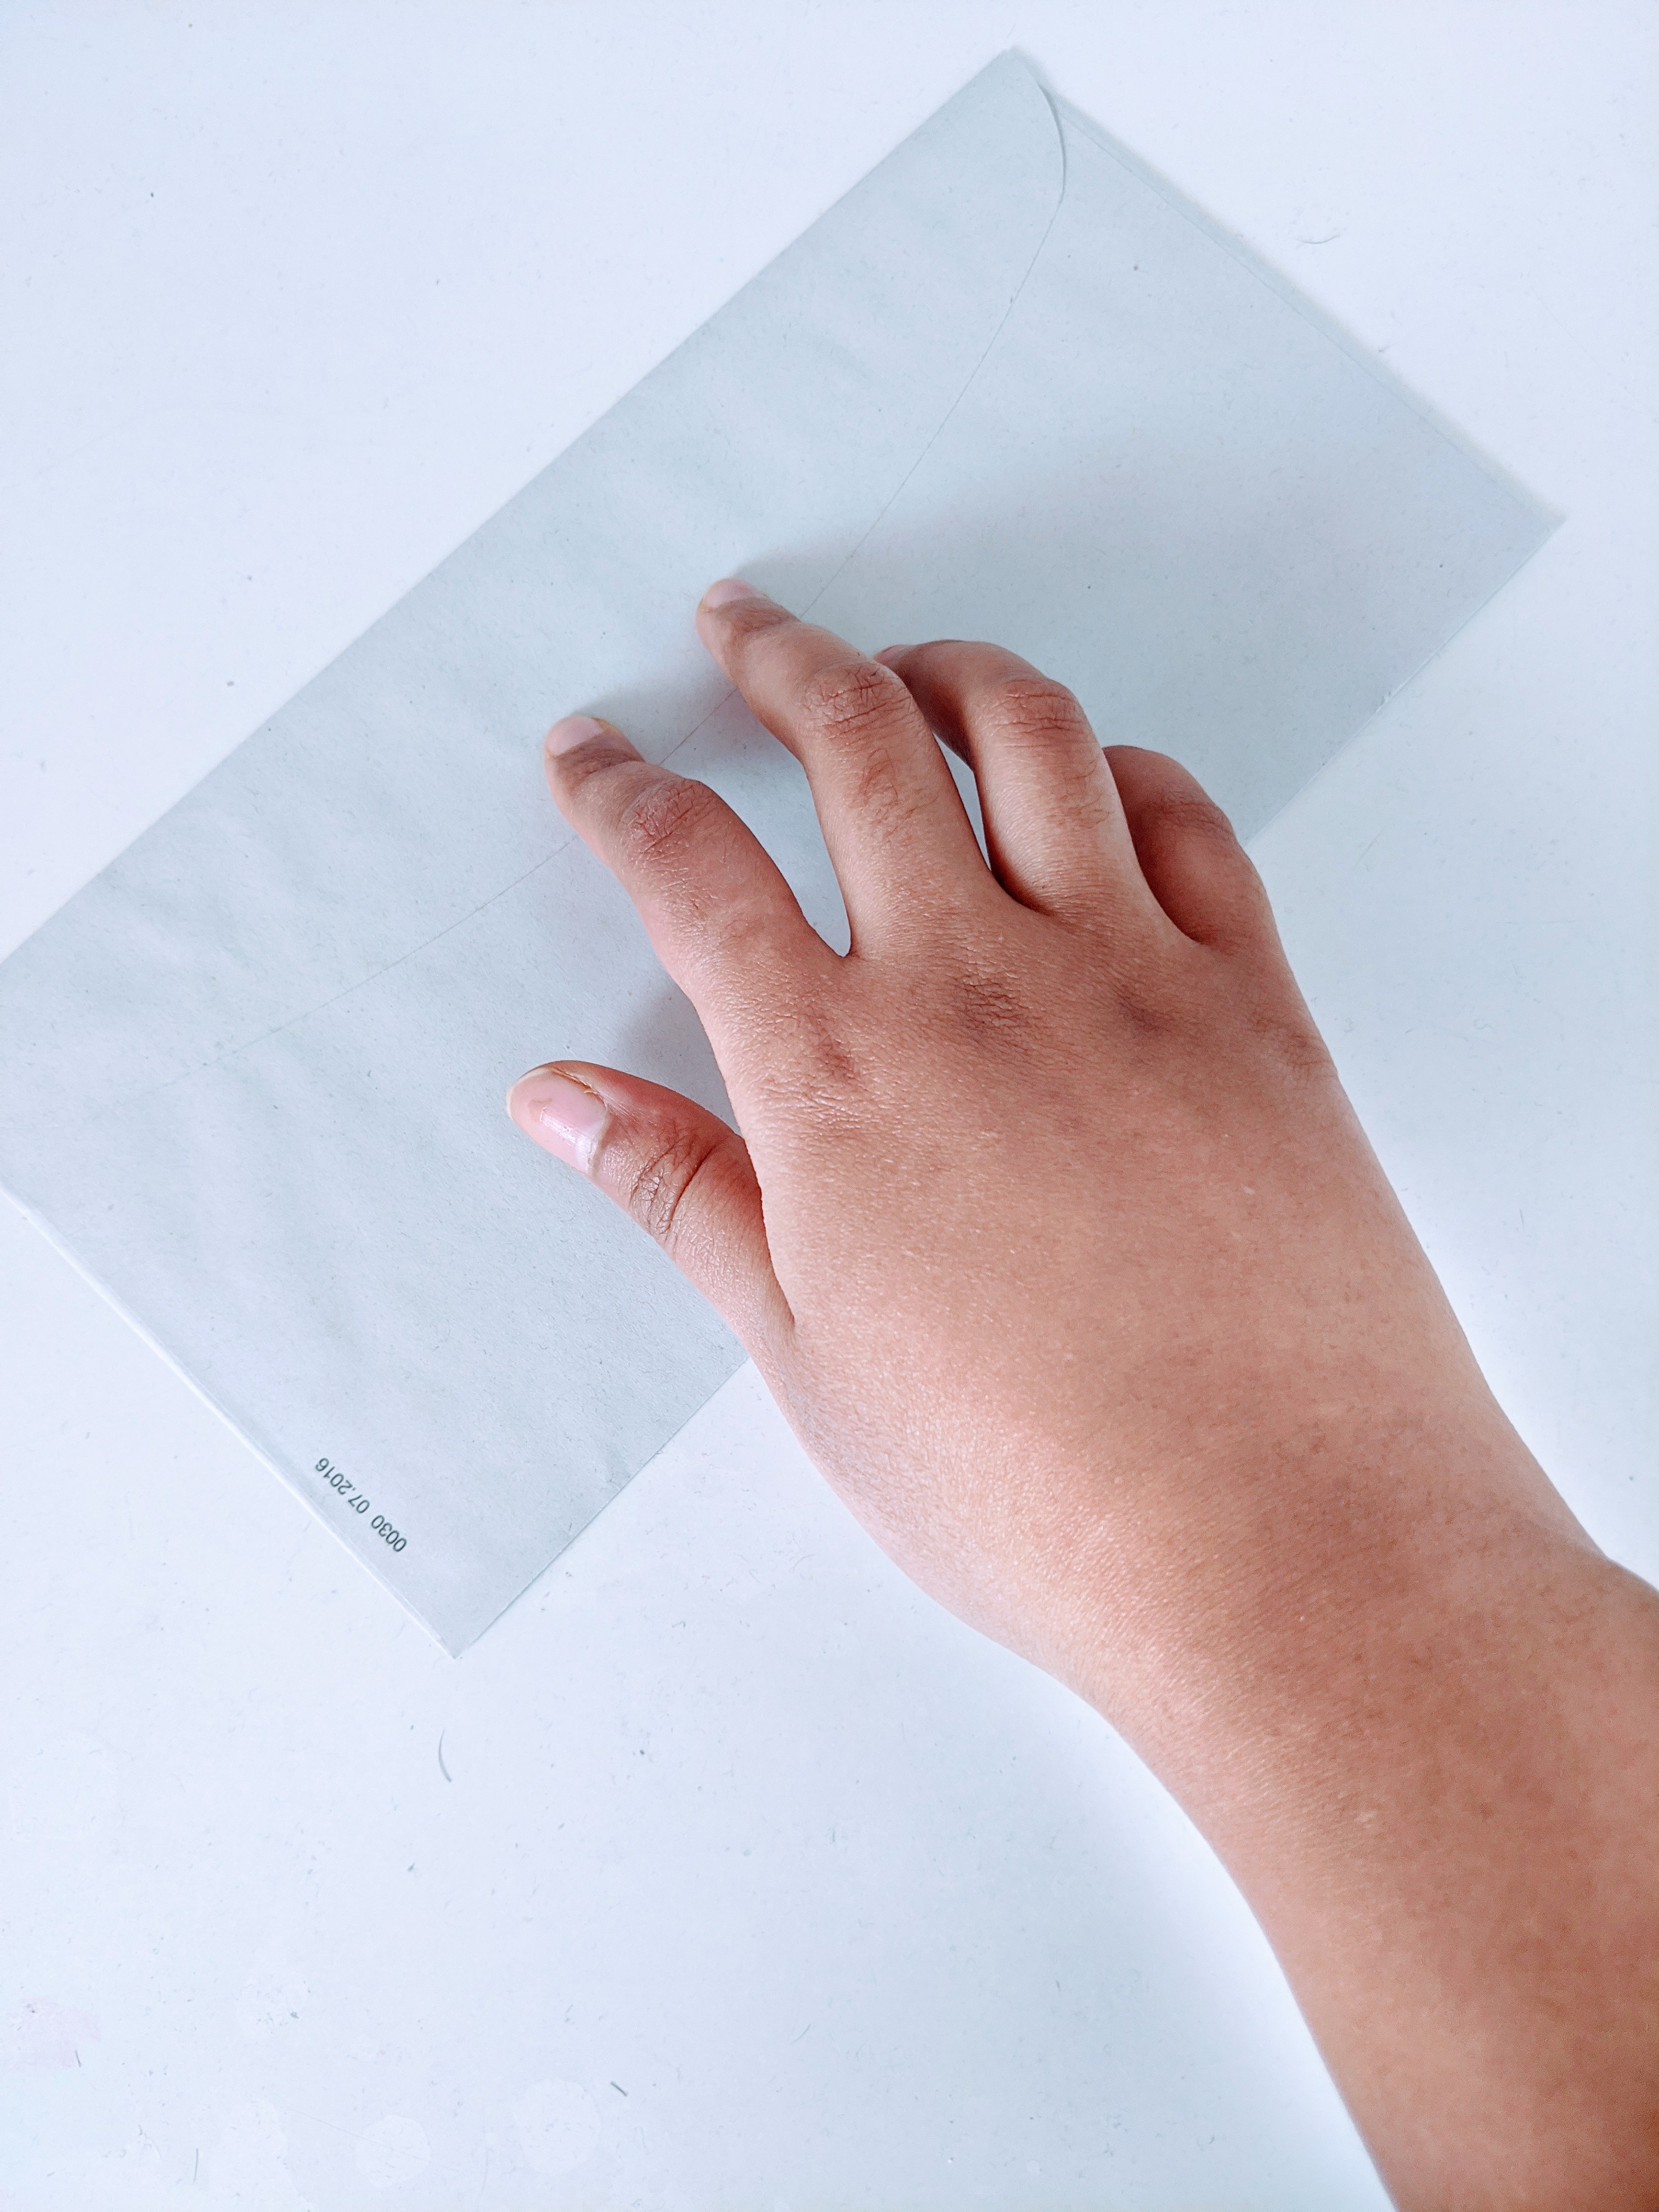
\includegraphics[scale=0.05]{images/env.jpg}
\caption{Intuitive and strategic positioning of hand on an envelope}
\label{env}
\end{center}
\end{figure}


Though an added complexity to this instance such as obstacles blocking the target object would make planning necessary to move the blocking obstacles on the way to create space for the target object as in \cite{dogar2011framework}, this approach does not relax such higher level planning that involves the order of obstacles to be moved. However, the lower level task of navigating the objects to desired location is motion-driven and not planning-driven. Transfer of such human behavior to robots offers advantages in several levels, such as faster performance, utilization of environmental setup, exploitation of available hardware. 

The above mentioned example can be logically broken down into following sub-problems;
\begin{itemize}
	\item Achieving the desirable finger configuration
	\item Establishing a compliant contact with the target object
	\item Moving the target object to target location
\end{itemize}
To achieve these tasks, few assumptions are made on the available knowledge to the system. The system does not include visual perception and the object geometric properties are assumed to be known. Also, the location of contact on/around the object is an input to the system.

The approaches involved in resolving each of the sub-tasks are explained below.

%\underline{\textbf{Selection of Desirable of Hand Configuration}} 
\paragraph{Selection of Desirable of Hand Configuration}~\\
As the idea behind the approach is to design and model human-inspired strategies, the finger configurations play a crucial role. To be able to handle a diverse sets of objects, three initial configurations are proposed in this work:
\begin{itemize}
	\item Single point contact
	\item Multi point contacts
	\item Line contact
\end{itemize}
As the name suggests, single point contact applies force on the top surface of the target object at a single point. With such contact, small objects such as an eraser, match box can be manipulated. Multi point contacts apply forces similarly at different points to achieve more stable control over the objects especially when they are flat or deformable, e.g. files, cards. The line contact applies provides more surface contact with one/more fingers almost wrapping the object. This helps in manipulating objects that are heavy or big such as books efficiently. The line contact configuration can also be applied when more than one object have to be handled. For instance, a pile of small screws can be swept away or gathered using this configuration. 


\paragraph{Establishment of Compliant Contact}~\\
The readings from the torque sensors of the manipulator joints can be utilized to sense the contact between the finger and the target object. Once the contact is established, required force parameter has to be updated to achieve stable caging of the object between the finger and its support surface. In case of line contact, compliance is relevant when hand is directly placed on the support surface. 


\paragraph{Motion of the Object to Desired Location}~ \\
Once a stable contact is achieved, a force is applied in desired direction on the surface until the object starts moving towards target location. For motion control, a simple control strategy can be applied (e.g PID).
\newpage
\section{Evaluation}

The method proposed in this work will be realised and demonstrated on two different use cases:
\begin{itemize}
\item Collection of objects on a table into a container (pushing as standalone manipulation)
\item Alignment of the objects on a table with given external contacts such as walls or surfaces of the table to eventually grasp with the support of external contacts (pushing as pre-grasp manipulation)
\end{itemize}

While the purpose of the demonstration on the use cases here is to signify the relevance and application of non-prehensile manipulation strategies, the use cases can further be used to measure the quality of the method in the task level. The following ideas can be considered to draw reasonable conclusions on the proposed solution.

\paragraph{Analysis of Approach on Unideal Objects}~\\
The objects considered during the demonstration can be varied to make the task more challenging to note the factors that influence failure of the approach. The idea is to change the geometric properties and/or position of the object itself to test if the method handles it. For instance, if the flat objects such as a book placed flat on the surface is successfully collected in the box, the method can be tested with even flatter objects such as a thin file, or a stack of papers. More examples include placing the book upright on the table, replacing flat objects by flat and deformable objects etc. This helps in analysing the ability of the approach to generalise over objects with different geometric properties. 

\paragraph{Analysis of Approach on Unideal Hardware}~\\
Though the approach is justifiable in ideal conditions, its high sensitivity to noisy hardware make it infeasible. Hence, relevant control signals that highly influence the proposed strategies can be identified during implementation and the signals can be used to analyse the robustness of the method. 


 \newpage
\section{Project Plan}


\begin{figure}[H]
 \begin{adjustwidth}{-1cm}{}
\begin{tabular}{|c|c|c|}

	\hline
	\multicolumn{2}{|c|}{\thead{Work Packages}} & \thead{Targeted date} \\
	\hline
	WP1 & Literature search & \\ [0.1ex]
	WP2 & State of the art analysis &  \\[0.2ex] \hline 
	\textbf{M1} & \textbf{Documentation of the state of the art} & 25-08-2020  \\
	\hline 
	WP3 & Design and modeling of finger configurations & \\ [0.1ex]
	WP4 & Implementation of the configurations on robot &   \\ [0.1ex]\hline
	\textbf{M2} & \textbf{Realisation of designed manipulation of strategies} &  20-10-2020 \\ 
	\hline
	WP5 & Implementation of pushing using the designed configurations &  \\ [0.1ex]
	WP6 & Integration of the method with compliant control&   \\[0.1ex] \hline
	\textbf{M3} & \textbf{Execution of compliant pushing using designed strategies} & 30-11-2020 \\
	\hline
	WP6 & Experimental evaluation of the solution on demo tasks & \\ [0.1ex]
	WP7 & Documentation of the experimental results &  \\[0.1ex] \hline
	\textbf{M4} & \textbf{Report submission} &  15-01-2021 \\
	\hline



\end{tabular}
	 \end{adjustwidth}
\end{figure}


\subsection{Project Schedule}

\begin{figure}[H]
    \begin{adjustwidth}{-1cm}{}
    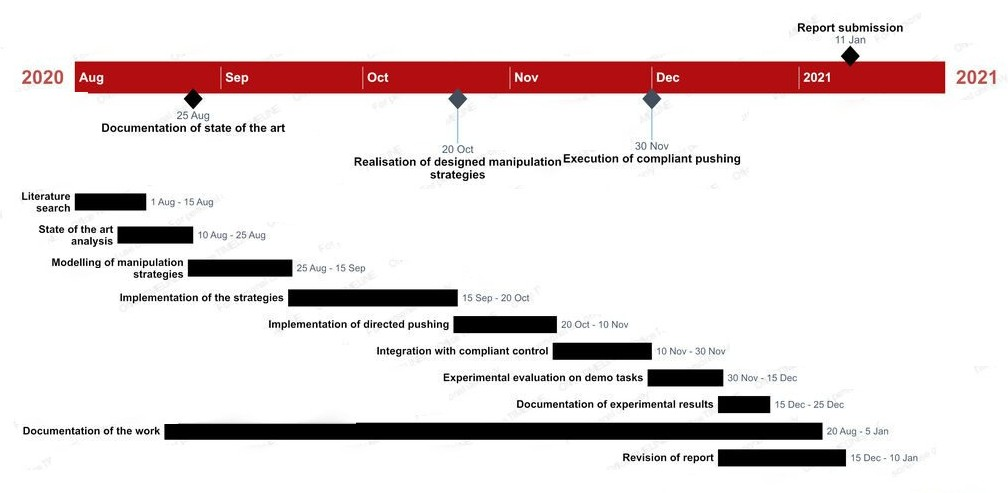
\includegraphics[width=18cm, height = 7.0cm]{gantt.jpg}
    \label{}
    \caption{Gantt chart representing distribution of tasks and milestones}
    	 \end{adjustwidth}
\end{figure}

\subsection{Deliverables}
\subsubsection*{Minimum Viable}

\begin{itemize}
    \item Literature survey and analysis of state of the art
    \item Design and modeling of finger configurations
    \item Realisation of the modeled configurations on robot 
\end{itemize}

\subsubsection*{Expected}
\begin{itemize}
	\item Implementation of compliant control
    \item Execution of directed pushing using the designed finger configurations
    \item  Demonstration of the solution on the task of aligning the objects with external contacts
\end{itemize}

 
\subsubsection*{Desired}
\begin{itemize}
   \item Demonstration of the proposed solution on the task of collecting the objects of interest into a container
\end{itemize}


\nocite{*}
\newpage
\bibliographystyle{plainnat} % Use the plainnat bibliography style
\bibliography{bibliography.bib} % Use the bibliography.bib file as the source of references




\end{document}
